% Architecture Description and system specifications
% 	* Multisensor IMS		
%		* Processing Stages
%		* Fusion approaches
%		* Methods and techniques
%		* Architecture proposal
%	* Validation approaches
%		* Transportation and Traffic Simulations
%			* Simulators Classification
%		* Intersection monitoring Datasets
%			* POSSi Dataset
%			* KoPER Dataset

%\chapter {Architecture Description and System Specification}
\chapter {System Description}

Although several types of sensors are used for intersection monitoring and supervision, the use of cameras, lasers and lidars has increased due to advances in sensors and computing capabilities. These enhancements have allowed to deploy more of these types of sensors per scenario and it is required to define some processing stages from raw data capture through decision and control. Also it is needed to test and validate the developments prior to a real and full functional implementation. The first part of this chapter describe main stages in a intersection management system based on image and range sensors, fusion approaches and methods used in these stages, and an architeture proposal for the implementation. In the second part, two validation tools for IMS applications are described, simulators and datasets.

\section{Multisensor IMS}

Multicamera and multilasers monitoring systems offer more information about environment that can be merged to provide a better representation of the whole scene, and to detect more acurately the objects in the intersection and prevent possible incidents. For designing an single-sensor or multi-sensor IMS system, there are some basic processing stages to have into account. In the case of a multisensor system, it is also required to analyse and determine what is the better fusion approach to use and in which of the processing stages this fusion should be performed, in order to get better results than a single-sensor based system. Below, processing stages, fusion approaches, methods and architecture proposal are presented.

\subsection{Processing Stages}

In the designing of an IMS, there are four main stages that have to be performed from the data source to final output: Filtering, feature extraction, pattern recognition and situation assessment. The aim of the first stage is to extract data of interest from the raw sensor information, using filtering and background subtraction techniques to get the foreground of the scene and remove noise and irrelevant data. In the second stage, the objective is to identify elements within the foreground and extract relevant features of them. The third stage receives the set of features from the previous stage and performs recognition and classification tasks. Also, tracking and prediction of objects' state is performed based on historic information. In the fourth stage, object behaviour and inter-objects interaction are analysed to identify context and detect situation or events of interest. This output could be delivered to an optional fifth stage of decision and control, to a human operator, or to a traffic agent or institution, for taking immediate actions on traffic control, issuing of traffic tickets, warning drivers about possible incidents or improving transportation policies in a long-term. In figure \ref{proc_stages}, are depicted the previously described stages, and how the data volume is reduced while data meaning increases in the last stages.

\begin{figure}[ht!]
\centering
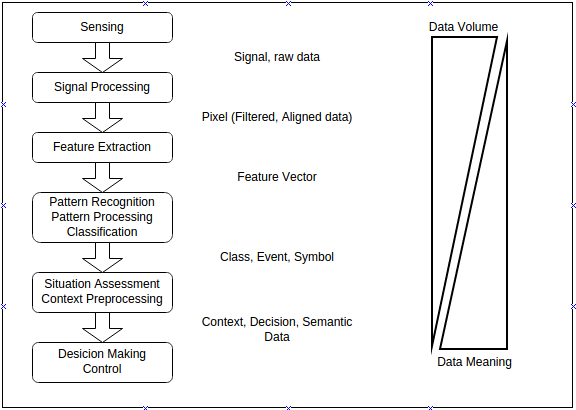
\includegraphics[scale=0.55]{fig/3/proc_stages.png}
\caption{Processing stages in an IMS.}
\label{proc_stages}
\end{figure}

\subsection{Fusion approaches}
\subsection{Methods and techniques}
\subsection{Architecture proposal}
\section{Validation approaches}
\subsection{Transportation and Traffic Simulations}
\subsubsection{Simulators Classification}
\subsection{Intersection monitoring Datasets}
\subsubsection{POSSi Dataset}
\subsubsection{KoPER Dataset}